\chapter{Testing and Application}

This chapter contains an overview of the testing performed for the development of \stops\ (\autoref{sec:test_stops}) and the checking of the replaced wavelength solutions (\autoref{sec:test_wav}), as well as the application of \stops\ on observations of both spectropolarimetric standards (\autoref{sec:specpol_stds}) and science targets (\autoref{sec:specpol_sci}).

% MARK: Test STOPS
\section[Testing \textsc{stops}]{Testing \stops} \label{sec:test_stops}

% No \polsalt\ tests or tests on pre-reduced \gls{FITS} files. (Trusted accurate)
% General discussion of testing (I.E. not this test was done specifically this source, more along the lines of these tests were done to check this issue, seen here using this source for example.)
The main challenge faced when developing \stops\ was ensuring that the software was compatible with both the \polsalt\ and \iraf\ file structures. As development is an iterative process, \stops\ was continually checked to ensure compatibility such that the varying \stops\ method inputs were correctly parsed, and that their outputs were parsable by the relevant \iraf\ tasks or \polsalt\ methods.

To this end, observations which were verified to have been accurately reduced were duplicated for testing purposes, allowing for continual checks of the \stops\ pipeline to be made during the development process. As the \stops\ \texttt{split} and \texttt{join} methods are designed to convert between the \polsalt\ and \iraf\ file structures, greater emphasis was made to ensure that the output of both methods provided accurate and consistent results.

% % Why the pipeline is better
% The rigorous error handling in \stops\ ensures that the user is informed of any issues that arise during the reduction process. This is particularly important as \stops\ was developed to enable a faster reduction process compared to that of pure \iraf\ or \polsalt.

% Reduction specific tests refer to tests performed to ensure no errant effects are introduced during the reduction process. These tests were designed to validate the accuracy and reliability of the \stops\ pipeline in producing scientifically accurate results.

% MARK: STOPS split tests
\subsection{Testing the \texttt{split} Method} \label{subsec:test_split}

The \stops\ \texttt{split} method requires any \polsalt\ pre-reduced (`mxgbp'- prefixed) \gls{FITS} files as input and outputs \iraf\ compatible (`(arc|beam)(O|E)'- prefixed) \gls{FITS} file structures. As no `split' \gls{FITS} files are created during pure \polsalt\ reductions, the \stops\ \texttt{split} method was tested by comparing the pre-reduced \polsalt\ files to the \texttt{split} method's output files, ensuring the correct structure and data integrity of the files handed off to \iraf.

% \newcommand\mc[1]{\multicolumn{1}{c|}{#1}} % handy shortcut macro

\begin{table}[t]

    \centering

    \caption{A comparison of the contents of a \polsalt\ pre-reduced \gls{FITS} file to the \stops\ \texttt{split} $O$- and $E$-beam \gls{FITS} files. Table created using the `\texttt{Astropy}' \texttt{fitsinfo} \gls{CLI} tool.}
    \label{table:split_info}

    \begin{tabular}{lcccccc}
        \toprule
        Filename &
        No. &
        Name &
        Type &
        Cards &
        Dimensions &
        Format \\
        \midrule
        \polsalt % mxgbpP201703280054.fits
        & $0$ & \gls{PRIMARY} & PrimaryHDU & $161$   & -                & -       \\
        & $1$ & \gls{SCI}     & ImageHDU   & $19$    & ($3199$, $1028$) & float32 \\
        & $2$ & \gls{VAR}     & ImageHDU   & $8$     & ($3199$, $1028$) & float32 \\
        & $3$ & \gls{BPM}     & ImageHDU   & $8$     & ($3199$, $1028$) & uint8   \\
        \stops\ \texttt{split} `$O$' % beamo0054.fits
        & $0$ & \gls{PRIMARY} & PrimaryHDU & $162$   & ($3199$, $474$)  & float32 \\
        \stops\ \texttt{split} `$E$' % beame0054.fits
        & $0$ & \gls{PRIMARY} & PrimaryHDU & $162$   & ($3199$, $474$)  & float32 \\ \bottomrule
    \end{tabular}

\end{table}


\autoref{table:split_info} shows the \gls{FITS} file information for the files before and after splitting. The split \gls{FITS} files contain the split \gls{SCI} extension data and the \gls{PRIMARY} header from the pre-reduced files, with any Header or Data differences mentioned below.

The header is left mostly untouched, and is only updated to represent the new data type and shape:
the `BITPIX' value is updated, from $8$ to $-32$, and the `NAXIS' value is updated, from $0$ to $2$;
the `NAXIS1' and `NAXIS2' keywords are added, and their values are set to the new split \gls{SCI} data shape;
and the `EXTEND' keyword is removed.%
\footnote{The `EXTEND' keyword indicates that the \gls{FITS} file contains multiple extensions while the `NAXIS1' and `NAXIS2' keywords indicate the shape and size of the data stored in the relevant extension.}
This accounts for the discrepancy in the `Cards' between the \polsalt\ and \stops\ file header entries in \autoref{table:split_info}.

\begin{figure}
    \centering
    \begin{subfigure}[b]{\textwidth}
        \centering
        
\includegraphics[width=\textwidth]{4_diff_O.pdf}
        \caption{The difference in the \gls{SCI} extensions, for the `O' polarization beam.}
        \label{subfig:diff_split_O}
    \end{subfigure}
    \hfill
    \begin{subfigure}[b]{\textwidth}
        \centering
        
\includegraphics[width=\textwidth]{4_diff_E.pdf}
        \caption{The difference in the \gls{SCI} extensions, for the `E' polarization beam.}
        \label{subfig:diff_split_E}
    \end{subfigure}
    \caption{The difference between the \polsalt\ pre-reduced (`mxgbp'- prefixed) \gls{FITS} files and the \stops\ `split' (`(arc|beam)(O|E)'- prefixed) files. Figures created using both the \polsalt\ \texttt{Raw image reduction} and \stops\ \texttt{split} method outputs.}
    \label{fig:split_diff}
\end{figure}

\autoref{fig:split_diff} shows that the \polsalt\ \gls{SCI} data is unmodified when copying the data to the \stops\ \gls{FITS} file, but only includes half of the data, for the relevant $O$- or $E$-polarization beam, \autoref{subfig:diff_split_O} and \autoref{subfig:diff_split_E}, respectively, with a cropping which defaults to $40$~pixels (see \autoref{subsec:stops_split}), introduced to the top- and bottom-most rows of the \polsalt\ data. This accounts for the discrepancy in the `Dimensions' between the \polsalt\ and \stops\ files in \autoref{table:split_info}.

This output file structure was chosen for \iraf\ compatibility, and was tested over multiple grating and articulation angles, as well as with various data sets to ensure that the \texttt{split} method was robust and reliable.

% MARK: STOPS join tests
\subsection{Testing the \texttt{join} Method} \label{subsec:test_join}

The \texttt{join} method requires both an \iraf\ database with wavelength solutions (or a custom wavelength solution) for both polarimetric beams and the \polsalt\ pre-reduced files as input and outputs \polsalt\ \texttt{spectra extraction} compatible (`wmxgbp'- prefixed) \gls{FITS} file structures. Ensuring that the output format was correct was paramount as the \polsalt\ \texttt{spectra extraction} method is unable to process the files otherwise, thus halting the reduction process. Thankfully, the \texttt{join} method output could be compared to the \polsalt\ \texttt{wavelength calibration} method output files, ensuring that any changes introduced by the \stops\ pipeline were well characterized.

\begin{table}[t]

    \centering

    \caption{A comparison of the \polsalt\ wavelength calibrated \gls{FITS} file to the (\iraf\ wavelength calibrated) \stops\ \texttt{join} \gls{FITS} file. Table created using the \texttt{Astropy} \texttt{fitsinfo} \gls{CLI} tool.}
    \label{table:join_info}

    \begin{tabular}{lcccccc}
        \toprule
        Filename &
        Ext. No. &
        Name &
        Type &
        Cards &
        Dimensions &
        Format \\
        \midrule
        \polsalt % wmxgbpP201703280054.fits
        & $0$ & \gls{PRIMARY} & Primary\gls{HDU} & $161$ & -             & -       \\
        & $1$ & \gls{SCI} & Image\gls{HDU} & $21$ & ($3199$, $514$, $2$) & float32 \\
        & $2$ & \gls{VAR} & Image\gls{HDU} & $10$ & ($3199$, $514$, $2$) & float32 \\
        & $3$ & \gls{BPM} & Image\gls{HDU} & $10$ & ($3199$, $514$, $2$) & uint8   \\
        & $4$ & \gls{WAV} & Image\gls{HDU} & $21$ & ($3199$, $514$, $2$) & float32 \\
        \stops\ \texttt{join} % wmxgbpP201703280054.fits
        & $0$ & \gls{PRIMARY} & Primary\gls{HDU} & $161$ & -             & -       \\
        & $1$ & \gls{SCI} & Image\gls{HDU} & $21$ & ($3199$, $474$, $2$) & float32 \\
        & $2$ & \gls{VAR} & Image\gls{HDU} & $10$ & ($3199$, $474$, $2$) & float32 \\
        & $3$ & \gls{BPM} & Image\gls{HDU} & $10$ & ($3199$, $474$, $2$) & uint8   \\
        & $4$ & \gls{WAV} & Image\gls{HDU} & $21$ & ($3199$, $474$, $2$) & float32 \\
        \bottomrule
    \end{tabular}

\end{table}


\autoref{table:join_info} shows the \gls{FITS} file information for both the \polsalt\ and \stops\ wavelength calibrated files. Other than the `Dimensions' of each `ImageHDU' extension,%
\footnote{The `Dimensions' differ due to the before mentioned cropping of the top- and bottom-most rows of the data.}
the \gls{FITS} files are identical in structure.

Although the `Cards' count is the same, minor differences across the headers are present. The `HISTORY' keyword, which contains the \polsalt\ `CRCLEAN' parameters and which default to `upper= 4.0, lower= 1.5, sigmaveto= 2.0', is left as `None' in the \stops\ file.%
\footnote{The \polsalt\ pipeline performs cosmic ray cleaning using a $10\sigma$ spike to cull cosmic rays. See the \polsalt\ \protect\href{https://github.com/saltastro/polsalt/blob/master/polsalt/specpolwavmap.py\#L132}{source code} for more information.}
Although \stops\ performs cosmic ray cleaning (see \autoref{subsec:stops_join}), the parameters are not stored in the header as \polsalt\ and \stops\ implement different methods for cosmic ray cleaning. Other minor differences such as the date-times stored in the `SAL-TLM' and `SMOSAIC' keywords may also differ as they contain the date-times relating to the completion of the \polsalt\ pre-reductions. This accounts for the differences in the `Cards' between the \polsalt\ and \stops\ file header entries in \autoref{table:join_info}.

\begin{figure}
    \centering
    \begin{subfigure}[b]{\textwidth}
        \centering
        
\includegraphics[width=\textwidth]{4_diff_SCI.pdf}
        \caption{The difference in the \gls{SCI} extensions.}
        \label{subfig:join_SCI}
    \end{subfigure}
    \hfill
    \begin{subfigure}[b]{\textwidth}
        \centering
        
\includegraphics[width=\textwidth]{4_diff_VAR.pdf}
        \caption{The difference in the \gls{VAR} extensions.}
        \label{subfig:join_VAR}
    \end{subfigure}
    \hfill
    \begin{subfigure}[b]{\textwidth}
        \centering
        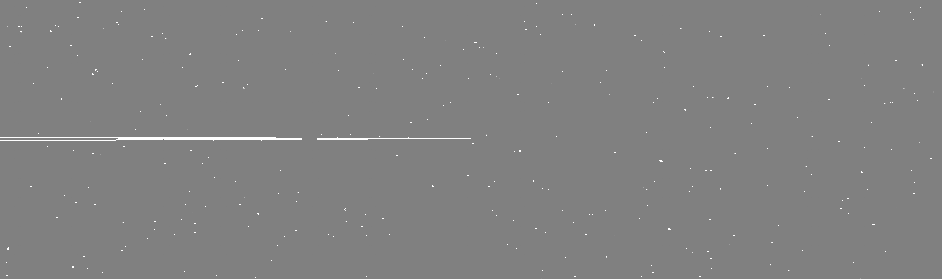
\includegraphics[width=\textwidth]{4_diff_BPM.pdf}
        \caption{The difference in the \gls{BPM} extensions.}
        \label{subfig:join_BPM}
    \end{subfigure}
    \hfill
    \begin{subfigure}[b]{\textwidth}
        \centering
        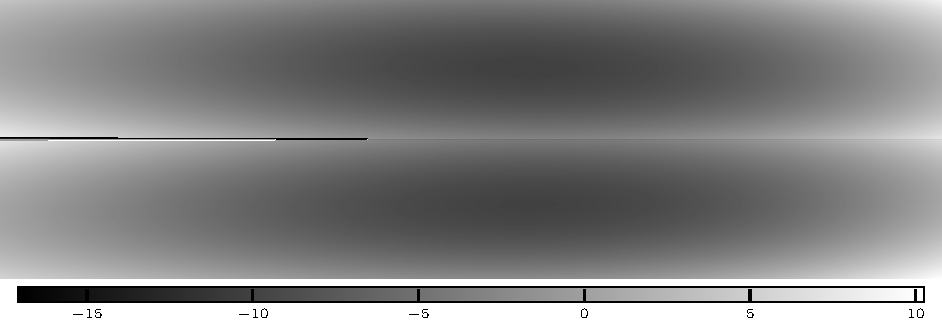
\includegraphics[width=\textwidth]{4_diff_WAV.pdf}
        \caption{The difference in the \gls{WAV} extensions.}
        \label{subfig:join_WAV}
    \end{subfigure}
    \caption{The difference of the \gls{FITS} file extensions between the \polsalt\ and \stops\ (`wmxgbp'- prefixed) wavelength calibrated files. Figures created using both the \polsalt\ and \stops versions of the \polsalt\ \texttt{spectral extraction} input.}
    \label{fig:join_in_out_diff}
\end{figure}

\autoref{fig:join_in_out_diff} shows the differences in the data between the \polsalt\ and \stops\ wavelength calibrated files. It can be seen that the \gls{VAR} extensions (\autoref{subfig:join_VAR}) are identical. The \gls{SCI} extensions (\autoref{subfig:join_SCI}) differ only in that the cosmic ray cleaning has been applied to the \stops\ data, whereas the \polsalt\ data applies a mask to the cosmic rays using the \gls{BPM} extension (\autoref{subfig:join_BPM}). The \gls{BPM} and \gls{WAV} extensions (\autoref{subfig:join_WAV}) are also masked to account for the valid wavelength calibrated region. The \gls{WAV} extensions contain the differing wavelength solutions and as such naturally differ. This accounts for the differences in the data between the \polsalt\ and \stops\ files.

Finally, the \stops\ \texttt{join} method was tested to ensure compatibility and correctness of the output data in comparison to \polsalt. This involved testing the \texttt{join} method with various data sets to ensure that the output files were accurate and consistent.

% MARK: Check Wav. Cal.'s
\section{Wavelength Solution Checks} \label{sec:test_wav}

% No \iraf\ tests or tests on \iraf\ \gls{FITS} files. (Trusted accurate)
The secondary challenge encountered when developing \stops\ was ensuring that the wavelength solutions parsed by \stops\ were unaffected by the pipeline and that they were similar to those created by \polsalt. This was achieved through the \texttt{correlate} and \texttt{skylines} methods, which were designed to validate the wavelength solutions produced by \iraf, but were later modified to parse both the \iraf\ and \polsalt\ wavelength solutions, allowing for further inspection of the two-dimensional wavelength solution.

Before the \polsalt\ wavelength calibrations were replaced with the \iraf\ wavelength calibrations, the accuracy of the new wavelength solutions needed to be validated. This was done both through the \iraf\ tasks, ensuring an accurate wavelength solution, and through the \stops\ \texttt{correlate} and \texttt{skylines} methods, allowing the integration of the wavelength solutions to be validated.

\todo{Add \gls{RMS} results (Table / Figures / Both?) from wavelength solution checks (\iraf\ \gls{RMS}, \polsalt\ \gls{RMS}) to quantify differences.}

\todo{Plot \iraf\ vs \polsalt\ \gls{RMS} for sources?}

% MARK: WAV Corr. Checks
\subsection{Cross Correlation Checks} \label{subsec:test_corr}

% O/E correlation checks to verify the consistency of the wavelength solutions.
The \texttt{correlate} method returns plots validating the wavelength solutions and so only has to accept the \polsalt\ \texttt{spectra extraction} (`ecwmxgbp'- prefixed) method output files as input.

\begin{figure}
    \centering
    \begin{subfigure}[b]{\textwidth}
        \centering
        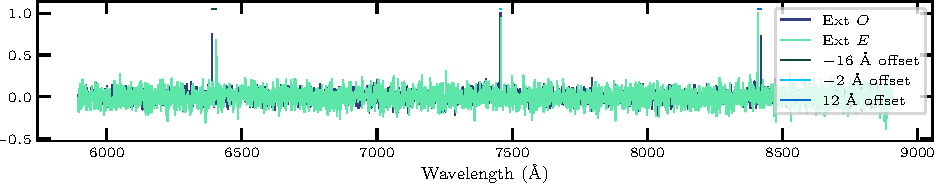
\includegraphics[width=\textwidth]{4_corr_spec.pdf}
        \caption{Generated $O$- and $E$-beam spectra.}
        \label{subfig:corr_test_spec}
    \end{subfigure}
    \hfill
    \begin{subfigure}[b]{\textwidth}
        \centering
        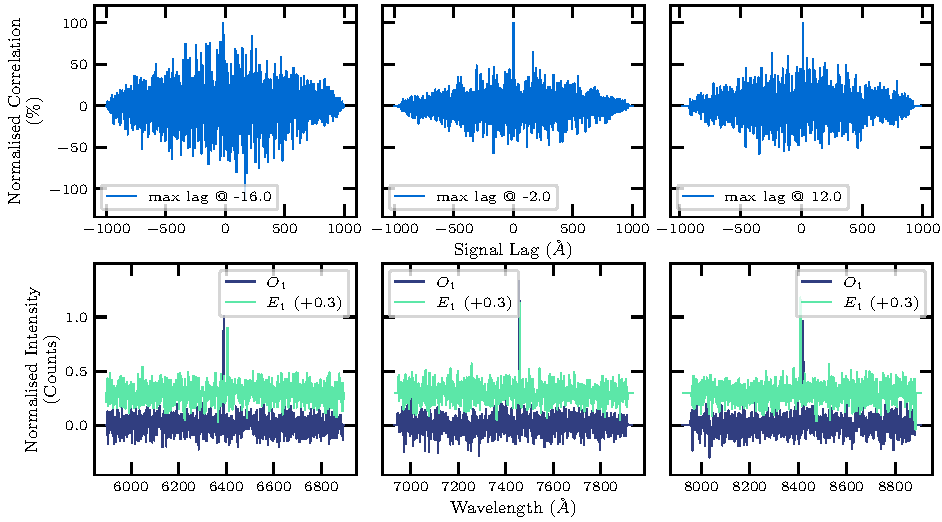
\includegraphics[width=\textwidth]{4_corr_test.pdf}
        \caption{The \stops\ \texttt{correlate} result for the spectra displayed in \subref{subfig:corr_test_spec}.}
        \label{subfig:corr_test_corr}
    \end{subfigure}
    \caption{Reacquisition of synthetic offsets introduced to the $O$- and $E$-beam spectra (\subref{subfig:corr_test_spec}) by cross-correlation (\subref{subfig:corr_test_corr}, bottom row).}
    \label{fig:corr_test}
\end{figure}

The \stops\ \texttt{correlate} method was tested by cross correlating generated $O$- and $E$-beam spectra with known offsets, with the aim of reacquiring said offsets, as shown in \autoref{fig:corr_test}. The spectra were generated with a feature in each \gls{CCD} region, randomly offset in both the wavelength and intensity axes, \autoref{subfig:corr_test_spec}.

Through cross correlation, \autoref{subfig:corr_test_corr}, the introduced offsets, or `max lag', were reacquired. For spectral regions with few features or features not much more significant than the continuum noise (such as the left most \gls{CCD} region of \autoref{subfig:corr_test_corr}), correlation may fail to determine the correct offset. It is clear that the returned `max lag' is incorrect when the `max lag' peak is not significantly larger than any noise of the continuum in the correlation plot.

% MARK: WAV Sky. Checks
\subsection{Sky Line Checks} \label{subsec:test_sky}

% Full frame wavelength solution checks to ensure comprehensive calibration.
% Verifying the accuracy of the cross-correlation function against known standards.
The \texttt{skylines} method returns plots validating the wavelength solutions and so only has to accept either the \iraf\ \texttt{transform} task or \stops\ \texttt{join} method output files as input.

\todo{Compare skylines from \stops\ to `poor' \polsalt\ spectral extraction (I.E. spectral extraction with no trace in the `target' window and the `background' window on region with no skylines).}

\todo{Test `skylines' using known spectral sky lines / telluric lines.}

\todo{Insert figure illustrating skyline identification accuracy.}

% MARK: Application
\section[Application of \textsc{stops}]{Application of \stops}
% https://ui.adsabs.harvard.edu/search/fq=%7B!type%3Daqp%20v%3D%24fq_database%7D&fq_database=database%3Aastronomy&p_=0&q=%20author%3A%22Cooper%2C%20J.%22%20spectropolarimetry&sort=date%20desc%2C%20bibcode%20desc

% Sources are blazars
The \stops\ pipeline has been utilized in the reduction of a number of sources, both for calibration tests using spectropolarimetric standards, and for science observations of transient blazars.

\begin{table}[t]
    \centering
    \begin{tabular}{cccccc}
        \toprule
        Source & \begin{tabular}[c]{@{}c@{}}Observation\\ Date\end{tabular} & Grating & \begin{tabular}[c]{@{}c@{}}Grating\\ Angle (\degree)\end{tabular} & \begin{tabular}[c]{@{}c@{}}Articulation\\ Angle (\degree)\end{tabular} & \begin{tabular}[c]{@{}c@{}}Exposure\\ Time (sec)\end{tabular} \\
        \midrule
        \multirow[t]{2}{*}{Hiltner 600} & \multirow[t]{2}{*}{2017-02-24} & \multirow[t]{2}{*}{PG0900} & $12.500$ & $24.91$ & $135.60$ \\
        &  &  & $19.625$ & $39.16$ & $135.60$ \\ % \cline{1-6}
        \multirow[t]{9}{*}{3C~279} & \multirow[t]{2}{*}{2017-03-28} & \multirow[t]{2}{*}{PG0900} & $12.498$ & $24.91$ & $480.81$ \\
        &  &  & $19.625$ & $39.16$ & $480.80$ \\ % \cline{2-6}
        & \multirow[t]{2}{*}{2017-04-01} & \multirow[t]{2}{*}{PG0900} & $12.500$ & $24.92$ & $480.78$ \\
        &  &  & $19.625$ & $39.17$ & $480.85$ \\ % \cline{2-6}
        & \multirow[t]{3}{*}{2017-05-17} & PG0300 & $5.375$ & $10.68$ & $720.84$ \\ % \cline{3-6}
        &  & \multirow[t]{2}{*}{PG0900} & $12.500$ & $24.92$ & $720.83$ \\
        &  &  & $19.625$ & $39.17$ & $901.05$ \\ % \cline{2-6}
        & 2017-05-21 & PG0300 & $5.375$ & $10.66$ & $1200.81$ \\ % \cline{2-6}
        & 2018-06-05 & PG0300 & $5.375$ & $10.72$ & $1200.81$ \\ % \cline{1-6}
        Hiltner 652 & 2022-06-10 & PG0900 & $12.878$ & $25.71$ & $\;\:48.50$ \\
        \bottomrule
    \end{tabular}

    \caption{Sources discussed from proceedings and publications within this section. Table adapted from \citet{cooper_HEASA2022}.}
    \label{table:sci_targets}

\end{table}


% MARK: spec. pol. std.'s
% \subsection{Spectropolarimetric Standards} \label{sec:specpol_stds}

% % Source | RA | DEC | Observation Date | Grating | Grating Angle | Articulation Angle | Exposure Time
\begin{table}[t]
    \centering
    \begin{tabular}{cccccccc}
        Source & RA                & DEC               & Observation Date & Grating & Grating Angle & Articulation Angle & Exposure Time \\ \hline
               &                   &                   &                  &         &               &                    &               \\ \hline
    \end{tabular}
    \caption{Spectropolarimetric standards discussed within this section.}
    \label{table:specpol_stds}
    \todo{Complete table of spectropolarimetric standards.}
\end{table}


% Spectropolarimetric standards must show little to no variability in both their spectroscopic and polarimetric properties. It is thus clear that blazars are not recommended as spectropolarimetric standards due to their high degree of variability.

% % Testing included the use of spectropolarimetric standards, comprising four highly polarized and two non-polarized objects. \todo{VERIFY CORRECT}

% \subsubsection{Source}

% \todo{For each standard:}

% \todo{Mention basic background information and a general discussion for source (A little more detail than included in paper).}

% \todo{General reduction steps performed (not necessary to constantly repeat self). Highlight any differences in reduction steps compared to science targets.}

% \todo{Insert figure(s) showing comparison plots of spectrum/polarization parameters from \polsalt\ and \stops (or leave out \polsalt\ and just show comparison to ($FORS1/2$) published results). Also short discussion (what the results can tell us and why it is useful). Focus on polarization results.}

% \todo{Add a `see \ ref{reference}' to final paragraph.}

% MARK: Science Targets
% \subsection{Spectropolarimetric Science Targets} \label{sec:specpol_sci}


\todo{Move to Introduction?}

The \stops\ pipeline has been utilized in the reduction of a number of science targets, specifically focused on blazars. Blazars are a subset of \gls{AGN} with relativistic jets closely aligned to our line of sight, and are known for their rapid and high degree of variability across the electromagnetic spectrum.

% What blazars are and how they are observed
Observations of these sources were performed using \gls{SALT}, specifically using the \gls{RSS} in spectropolarimetry mode (\autoref{sec:RSS_reductions}). \gls{SALT}, and more specifically the \gls{RSS} grating used (\autoref{table:RSS_gratings}), limits the wavelength range to the optical and \gls{NIR} regions. This allows for the study of the polarization properties of blazars within these wavelength regimes, which are often dominated by a polarized, non-thermal emission component arising in the jets, with an underlying non-polarized, thermal emission component arising from the host galaxy, dusty torus, and accretion disk components.

% MARK: HEASA 2021
\subsubsection[Development of \textsc{stops}: Application to the blazar 3C 279]{Development of Tools for the \gls{SALT}/\gls{RSS} Spectropolarimetry Reductions:\\Application to the Blazar 3C 279\hfill(Proceedings of Science, \glsxtrshort{HEASA} 2021)}

% Basic background information
In \cite[][see also \autoref{app:papers}]{cooper_HEASA2021}, it was shown that alternative wavelength solutions, such as those created using \iraf, are capable of being applied to \gls{SALT} spectro\-polarimetric data. The `additional tools' mentioned therein, which were the precursor to the \stops\ pipeline, were used for the reduction of the blazar $3$C~$279$.

The blazar $3$C~$279$ was observed in linear spectropolarimetry mode, on $2017$ May $17$, using the PG$0900$ grating with two different grating angles ($12.5$\degree\ and $19.5$\degree). The grating and articulation angles used for the observations, as shown in \autoref{table:sci_targets}, matched those of observations of the spectrophotometric standard star, Hiltner $600$, observed on $2017$ February $24$, allowing the intensity to be relatively flux calibrated.

\begin{figure}[t]
    \centering
    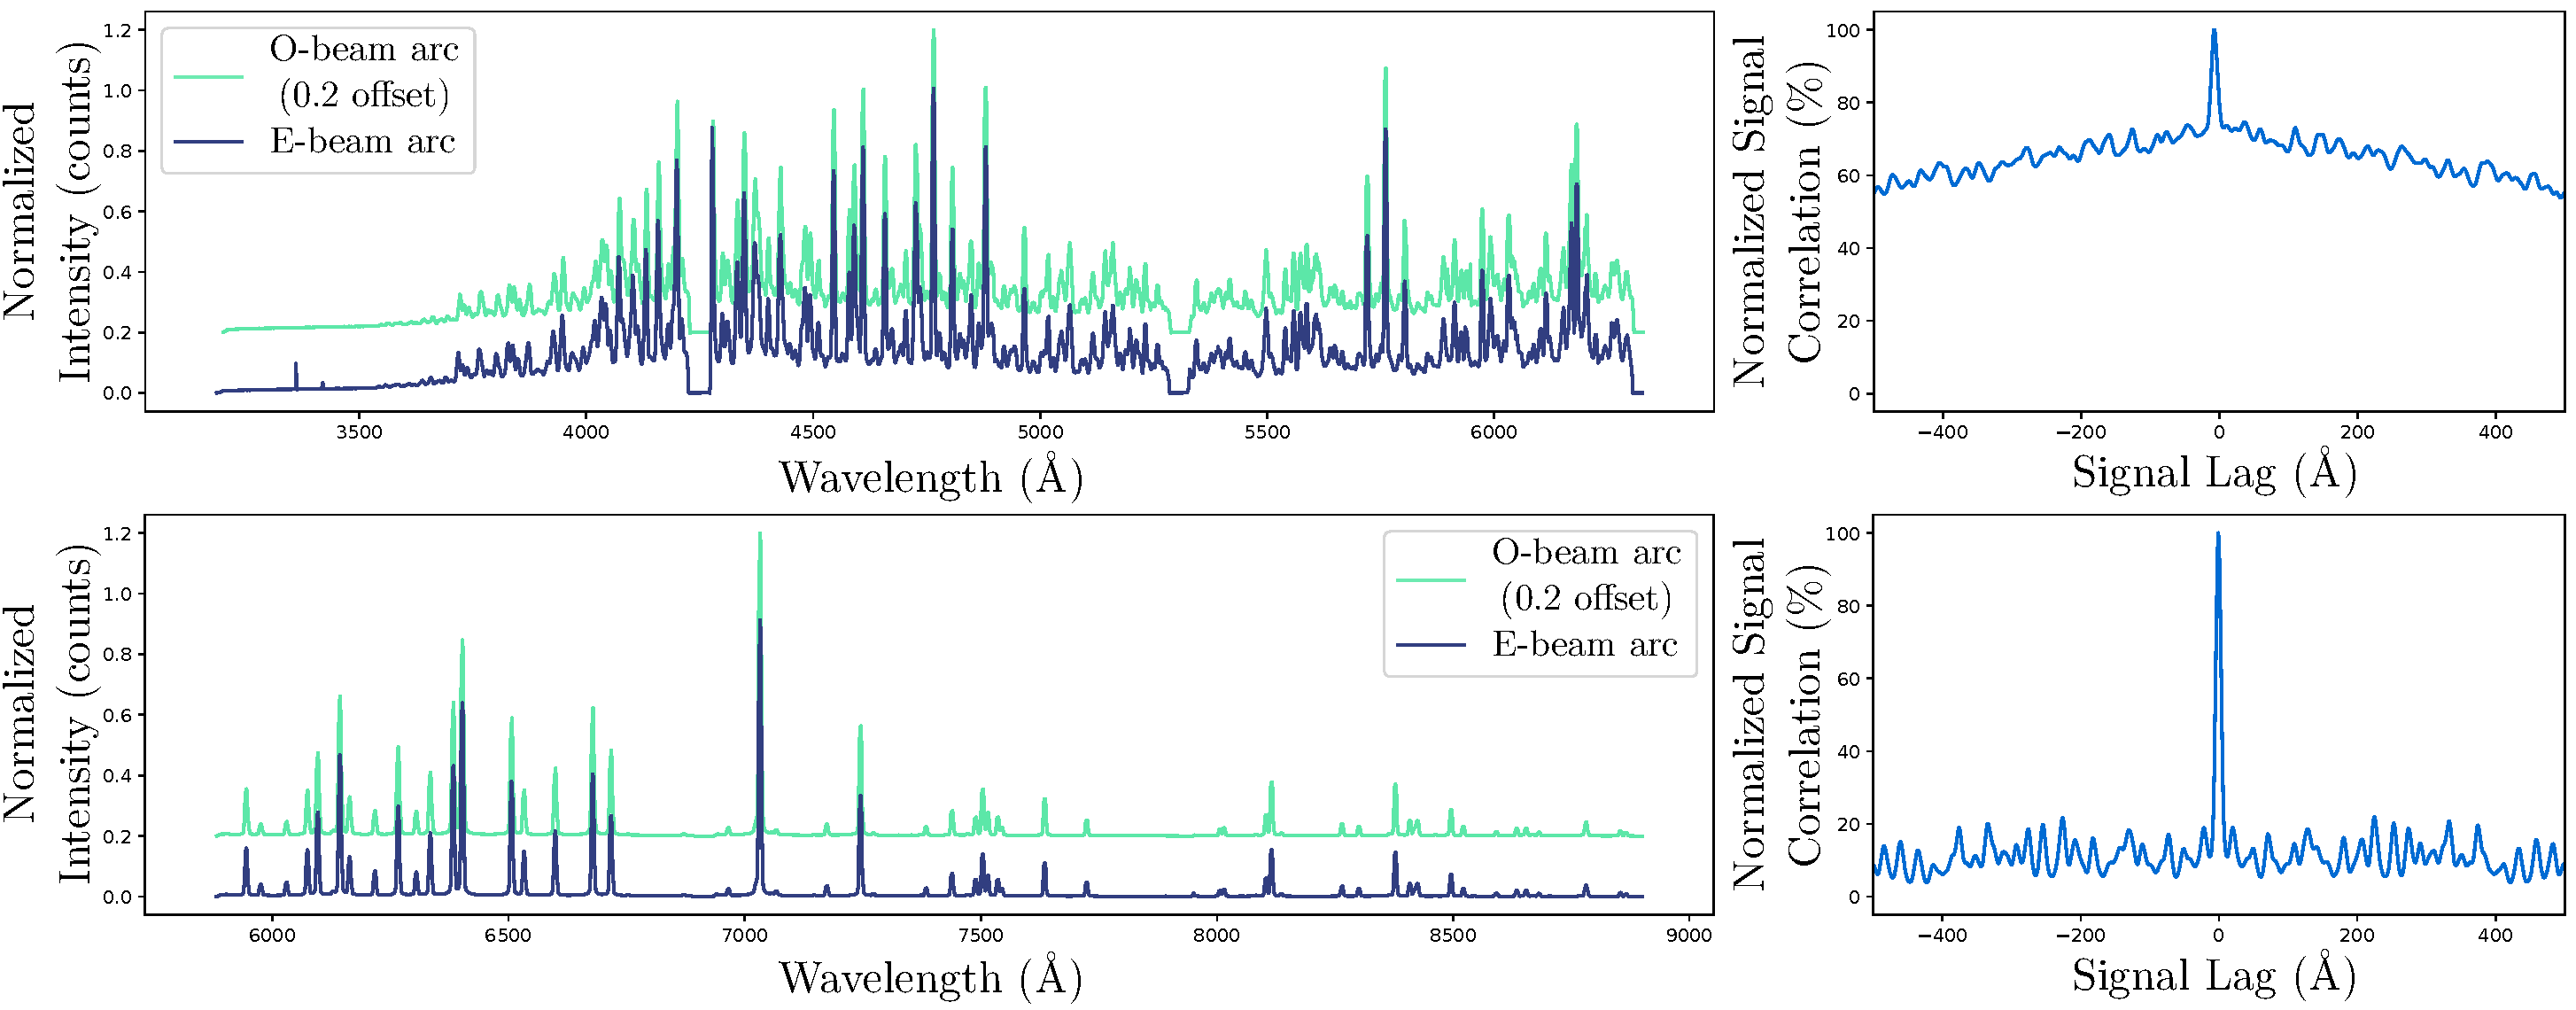
\includegraphics[width = 1.0\textwidth]{4_HEASA2021_oecorr.pdf}
    \caption{The spectra and cross correlation of the $O$- and $E$-beams of the \gls{ThAr} (top) and \gls{NeAr} (bottom) arc lamps. Figure adapted from \citep{cooper_HEASA2021}.}
    \label{fig:HEASA2021_oecorr}
\end{figure}

\autoref{fig:HEASA2021_oecorr} shows the spectra and cross correlation of the $O$- and $E$-beams of the \gls{ThAr} and \gls{NeAr} arc lamps, with grating angles of $12.5$\degree\ and $19.5$\degree, respectively. The cross correlation of the arc lamps perpendicular polarization beams show clear peaks at $0$ lag, indicating that the wavelength solutions are consistent across the two polarization beams.

\begin{figure}[t]
    \centering
    \begin{subfigure}[b]{1.0\textwidth}
        \centering
        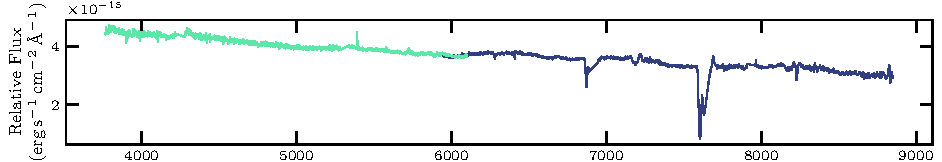
\includegraphics[width = 1.0\textwidth]{4_HEASA_2021_spec.pdf}
        \caption{The relative flux calibration of the $3$C~$279$ spectra.}
        \label{subfig:HEASA2021_spec}
    \end{subfigure}
    \hfill
    \begin{subfigure}[b]{1.0\textwidth}
        \centering
        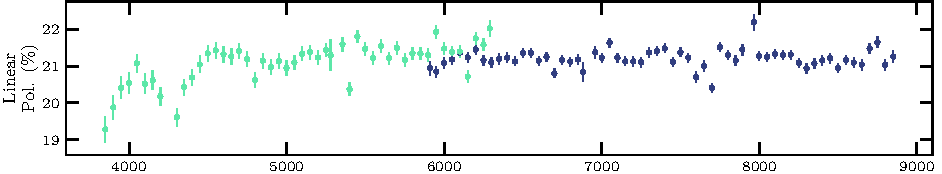
\includegraphics[width = 1.0\textwidth]{4_HEASA_2021_pol.pdf}
        \caption{The linear polarization percentage of the $3$C~$279$ spectra.}
        \label{subfig:HEASA2021_pol}
    \end{subfigure}
    \hfill
    \begin{subfigure}[b]{1.0\textwidth}
        \centering
        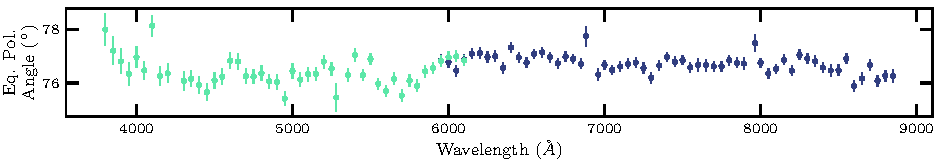
\includegraphics[width = 1.0\textwidth]{4_HEASA_2021_pol_ang.pdf}
        \caption{The polarization angle of the $3$C~$279$ spectra, polarization relative to the instrument.}
        \label{subfig:HEASA2021_pol_ang}
    \end{subfigure}
    \caption{The relative flux calibrated spectra (\subref{subfig:HEASA2021_spec}), linear polarization percentage (\subref{subfig:HEASA2021_pol}), and polarization angle (\subref{subfig:HEASA2021_pol_ang}) of the blazar $3$C~$279$ observed on $2017$ May $17$. Figure adapted from \cite{cooper_HEASA2021}.}
    \label{fig:HEASA2021}
\end{figure}

\autoref{fig:HEASA2021} shows the relative flux calibrated intensity, percentage of linear polarization, and polarization angle of the blazar $3$C~$279$, across the visible spectrum. The spectra show a good overlap between the two grating angles, especially when considering the variable nature of blazars. Both the percentage of linear polarization and the polarization angle generally agree across the grating angle overlap.

% MARK: HEASA 2022
\subsubsection[SALT Spectropolarimetric Pipeline Comparisons]{\gls{SALT} Spectropolarimetric Pipeline Comparisons\\\strut\hfill(Proceedings of Science, \glsxtrshort{HEASA} 2022)}

As discussed in \cite[][see also \autoref{app:papers}]{cooper_HEASA2022}, \todo{\dots}

% MARK: Buckley 191221B
\subsubsection{Spectropolarimetry and Photometry of the Early Afterglow of the Gamma-ray Burst GRB~191221B\hfill\mbox{\citep{Buckley191221B}}}


% MARK: Schutte - 4C+01.02
\subsubsection{Modeling the Spectral Energy Distributions and Spectropolarimetry of Blazars - Application to 4C+01.02 in 2016 - 2017\hfill\citep{Schutte4C0102}}

% Mention basic background information
% Provide a general discussion for source (summary of paper + necessary extra).

% Provide the general reduction steps performed, if unique.

% Insert figure(s) showing comparison plots of spectrum/polarization parameters from \polsalt\ and \stops (or leave out \polsalt\ and just show published results).

% Also short discussion (what the results can tell us and why it is useful).
% Focus on polarization results.
